\documentclass[11pt,a4paper]{article}
\usepackage[margin=25mm]{geometry}
\usepackage[T1]{fontenc}
\usepackage{lmodern,microtype,amsmath,amssymb,amsthm,mathtools,booktabs,graphicx}
\usepackage{xcolor,enumitem,fancyhdr,tikz}
\usetikzlibrary{arrows.meta,positioning,calc}
\definecolor{ink}{HTML}{41304F}
\definecolor{link}{HTML}{356C69}
\definecolor{hot}{HTML}{B4442E}
\definecolor{cold}{HTML}{2E6DB4}
\usepackage[colorlinks=true,linkcolor=link,citecolor=link,urlcolor=link]{hyperref}
\hypersetup{pdftitle={Thermal heat-current cumulant ratios can be arbitrarily negative},pdfauthor={Anonymous}}
\newtheorem{theorem}{Theorem}[section]
\newtheorem{proposition}[theorem]{Proposition}
\newtheorem{lemma}[theorem]{Lemma}
\newtheorem{corollary}[theorem]{Corollary}
\theoremstyle{remark}\newtheorem{remark}[theorem]{Remark}
\newcommand{\eps}{\varepsilon}
\newcommand{\E}{\mathbb E}
\setlength{\parskip}{4pt}
\setlength{\parindent}{0pt}
\pagestyle{fancy}\fancyhf{}
\fancyhead[L]{\small\textcolor{ink}{Thermal current cumulants}}
\fancyhead[R]{\small Version 2.0, 27 October 2026}
\fancyfoot[C]{\thepage}
\setlength{\headheight}{14pt}
\makeatletter
\renewcommand{\@maketitle}{\newpage\begin{center}
{\LARGE\@title\par}\vspace{0.8em}{\large\@author\par}\vspace{0.4em}{\small\@date\par}
\end{center}\vspace{0.8em}}
\makeatother
\title{\textcolor{ink}{Thermal heat-current cumulant ratios can be arbitrarily\\negative: three-state counterexamples to two sign conjectures}}
\author{Anonymous}
\date{27 October 2026\quad\textnormal{\small Version 2.0, release 1.0.0-candidate\\ \url{https://doi.org/10.5281/zenodo.23689958}}}
\begin{document}
\maketitle
\begin{abstract}
Ptaszy\'nski (2022) conjectured, on the basis of random-network calculations, that the normalised third and fourth heat-current cumulant ratios $C_3/C_1$ and $C_4/C_2$ are nonnegative in classical Markov systems driven only by temperature differences. A negative value could then have certified non-thermal or non-classical driving. We give exact three-state counterexamples that obey local detailed balance with two baths. After a common rescaling of all rates, which leaves both ratios unchanged, a fully connected family keeps the energies, temperatures, stationary probabilities, mean heat current and entropy production fixed while both ratios tend to $-\infty$ like $\eps^{-2}$. In the standard state-jump model with one counted bath, two states can never violate either sign. The mechanism is classical slow switching, and the divergence tracks the variance, which grows like $\eps^{-1}$: the variance-normalised ratios $C_3C_1/C_2^2$ and $C_4C_1^2/C_2^3$ tend to $-9/4$ and $-3/4$. Variance-based bounds such as the thermodynamic uncertainty relation are untouched. For positive mean and variance we prove a kinetic lower bound, in terms of the spectral separation of the stationary eigenvalue, that captures the $\eps^{-2}$ rate. We also show that variance normalisation alone does not restore a bound: with six states both normalised ratios are unbounded below at fixed energies and temperatures. Violations need rate separations of order $10^2$ (a disparity above $60$ suffices in the simplest example), which is why random sampling rarely finds them. The practical message is that a negative ratio does not certify quantum or non-thermal driving; slow switching must be excluded first.
\end{abstract}

\section{Introduction}\label{sec:intro}
\paragraph{What is being measured.} A small conductor placed between a hot and a cold reservoir passes heat in random bursts. Over a long time $t$ the delivered heat $Q_t$ has cumulants that grow linearly in $t$; their rates $C_n$ summarise the statistics. $C_1$ is the mean heat current and $C_2$ its noise. $C_3$ measures lopsidedness: it is positive when the record is dominated by rare large bursts above the mean, and negative when it is dominated by rare shortfalls. $C_4$ measures how heavy both tails are compared with Gaussian noise.

\paragraph{Why positivity was expected.} The thermodynamic uncertainty relation~\cite{BaratoSeifert2015,Gingrich2016} bounds the noise $C_2$ from below by the dissipation. Higher cumulants have been studied in the same spirit~\cite{BaratoSeifert2015sk,WamplerBarato2022,Salazar2022}. Ptaszy\'nski~\cite{Ptaszynski2022} found that in more than $30\,000$ random classical networks driven only by temperature differences, the ratios
\begin{equation}\label{eq:ratios0}
S=\frac{C_3}{C_1},\qquad K=\frac{C_4}{C_2}
\end{equation}
were never negative. He conjectured that $K\ge0$ always holds, and $S\ge0$ for one temperature difference (his equations (19)--(20)). He noted that a violation could then be used to infer forces other than temperature differences. A sign rule would have been a cheap diagnostic: measure two higher cumulants and learn whether a device is driven by something beyond heat.

\paragraph{Answer.} The conjectures are false, and with three states. A conductor that occasionally falls into a long-lived idle state, as in Figure~\ref{fig:schematic}, produces a current that switches between ``on'' and ``off''. When the idle state is entered rarely and left slowly, the long-time statistics are those of a telegraph signal, and $C_3$ and $C_4$ become large and negative. This mechanism is classical~\cite{Jordan2004,BagretsNazarov2003}, and switching between current-carrying states also appears in recent thermal work~\cite{PtaszynskiEsposito2025}. What is new is its exact realisation inside the conjectured class, the strengthening to fixed thermodynamic data, and an account of what can still be bounded.

\begin{figure}[tb]
\centering
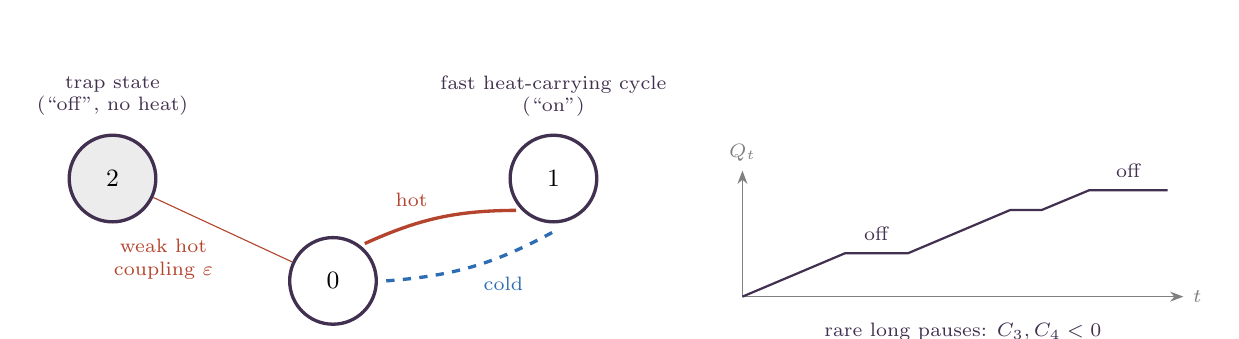
\begin{tikzpicture}[>=Stealth,node distance=2.6cm,
  st/.style={circle,draw=ink,very thick,minimum size=11mm,font=\small},
  hotl/.style={hot,very thick},coldl/.style={cold,very thick,dashed}]
\node[st] (s0) at (0,0) {$0$};
\node[st] (s1) at (2.8,1.3) {$1$};
\node[st,fill=gray!15] (s2) at (-2.8,1.3) {$2$};
\draw[hotl] ([yshift=2pt]s0.north east) to[bend left=12] node[above left,font=\scriptsize]{hot} ([xshift=-2pt]s1.south west);
\draw[coldl] ([xshift=3pt]s0.east) to[bend right=12] node[below right,font=\scriptsize]{cold} ([yshift=-3pt]s1.south);
\draw[hotl,thin] (s0) -- node[below left,font=\scriptsize,align=center]{weak hot\\coupling $\eps$} (s2);
\node[font=\scriptsize,align=center,text=ink] at (2.8,2.35) {fast heat-carrying cycle\\(``on'')};
\node[font=\scriptsize,align=center,text=ink] at (-2.8,2.35) {trap state\\(``off'', no heat)};
% telegraph trace
\begin{scope}[shift={(5.2,-0.2)}]
\draw[->,gray] (0,0) -- (5.6,0) node[right,font=\scriptsize]{$t$};
\draw[->,gray] (0,0) -- (0,1.6) node[above,font=\scriptsize]{$Q_t$};
\draw[ink,thick] (0,0) -- (1.3,0.55) -- (2.1,0.55) -- (3.4,1.1) -- (3.8,1.1) -- (4.4,1.35) -- (5.4,1.35);
\node[font=\scriptsize,text=ink] at (1.7,0.8) {off};
\node[font=\scriptsize,text=ink] at (4.9,1.6) {off};
\node[font=\scriptsize,text=ink,align=center] at (2.8,-0.45) {rare long pauses: $C_3,C_4<0$};
\end{scope}
\end{tikzpicture}
\caption{The weak-trap mechanism. States $0$ and $1$ form a fast cycle that carries heat from the hot bath (solid) to the cold bath (dashed). State $2$ is a trap reached only through a weak hot-bath edge that carries no heat. The heat record (right, schematic) alternates between steady flow and long pauses. Rare long pauses skew the record towards shortfalls.}
\label{fig:schematic}
\end{figure}

\paragraph{Roadmap.} Section~\ref{sec:defs} fixes the setting and checks it against the source hypothesis by hypothesis. Section~\ref{sec:simple} gives a small exact certificate. Section~\ref{sec:trap} proves the general weak-trap asymptotics. Section~\ref{sec:full} removes degenerate features and holds the thermodynamic data fixed. Section~\ref{sec:normalised} asks what survives: variance-normalised ratios and a kinetic bound. Section~\ref{sec:minimal} shows that two states never suffice. Section~\ref{sec:practice} explains why random sampling missed the effect and what an experiment would need. Section~\ref{sec:verify} describes the exact verification, and Section~\ref{sec:open} lists open problems.

\paragraph{Scope.} We claim no novelty for slow-switching statistics, for differentiating characteristic polynomials~\cite{Bruderer2014}, or for two-state counting formulas. Our search for prior resolutions (Semantic Scholar citation graph of~\cite{Ptaszynski2022}, Crossref and general web search, completed 27 October 2026) found three citing works, none addressing equations (19)--(20). That cannot establish absolute priority.

\section{Setting and the conjectured class}\label{sec:defs}
Consider a finite continuous-time Markov chain with state energies $E_i$, in units with $k_B=1$. Write $k^\alpha_{ij}$ for the rate of the jump $j\to i$ caused by bath $\alpha\in\{h,c\}$. Local detailed balance reads
\begin{equation}\label{eq:ldb}
k^\alpha_{ij}/k^\alpha_{ji}=\exp[-\beta_\alpha(E_i-E_j)],\qquad\beta_\alpha>0.
\end{equation}
A cold-bath jump $j\to i$ delivers heat $E_j-E_i$ to the cold bath; a hot-bath jump delivers none to it. With column probability vectors the tilted generator is
\begin{equation}\label{eq:tilt}
[L(z)]_{ij}=k^h_{ij}+k^c_{ij}e^{z(E_j-E_i)}\ (i\ne j),\qquad[L(z)]_{jj}=-\textstyle\sum_{i\ne j,\alpha}k^\alpha_{ij}.
\end{equation}
For an irreducible chain $0$ is a simple eigenvalue of $L(0)$; its analytic continuation $\chi(z)$ is the scaled cumulant generating function of $Q_t$, and $C_n=\chi^{(n)}(0)$. The ratios~\eqref{eq:ratios0} carry units of energy squared. They are unchanged by reversing the counted heat and by multiplying all rates by a common constant. For two baths the mean entropy-production rate is $\dot\sigma=(\beta_c-\beta_h)C_1$, so it is not independent data.

Table~\ref{tab:hyp} compares this setting with the source. The source counts heat into bath $\alpha$ with the same tilting~\eqref{eq:tilt} (its equation (67)), so its $S_h$ and $K_h$ coincide with our $S$ and $K$.
\begin{table}[tb]\centering\small
\begin{tabular}{p{0.45\textwidth}p{0.45\textwidth}}
\toprule
Hypothesis in~\cite{Ptaszynski2022}, Sec.~III (stated) and III D (setting) & Where it holds here\\
\midrule
Finite classical continuous-time Markov chain & All examples; irreducible for $\eps>0$\\
Rates are sums over baths, $k_{ij}=\sum_\alpha k^\alpha_{ij}$ (eq.~65); parallel bath channels allowed & Sec.~\ref{sec:full}: every pair coupled to both baths\\
Bathwise local detailed balance (eq.~66), otherwise arbitrary rates & Checked edge by edge, Secs.~\ref{sec:simple}, \ref{sec:full}\\
Driving by temperature differences only; single difference for (20) & Two baths, no chemical or mechanical force\\
Heat current into one bath, counting field as in eq.~67 & Cold-bath current~\eqref{eq:tilt}\\
\bottomrule
\end{tabular}
\caption{The counterexamples satisfy every hypothesis of the conjectures.}\label{tab:hyp}
\end{table}

\section{A small exact certificate}\label{sec:simple}
Take $E=(0,1,0)$, $\beta_h=\log2$, $\beta_c=\log4$. On the pair $0\leftrightarrow1$ the hot up/down rates are $1,2$ and the cold up/down rates are $1,4$. State $2$ is the trap: it is joined to state $0$ by a hot edge with equal rates $\eps$ in both directions. This edge has zero energy change, so it carries no heat; this degeneracy is removed in Section~\ref{sec:full}. Then $\pi=(3,1,3)/7$ and
\begin{equation}
L(z)=\begin{pmatrix}-2-\eps&2+4e^z&\eps\\1+e^{-z}&-6&0\\\eps&0&-\eps\end{pmatrix},
\end{equation}
\begin{equation}
\det(xI-L(z))=x^3+(8+2\eps)x^2+14\eps x-\{4(e^z-1)+2(e^{-z}-1)\}(x+\eps).
\end{equation}
Differentiating $\det(\chi(z)I-L(z))=0$ at $z=0$ gives
\begin{align}
C_1&=\frac17,& C_2&=\frac{6+145\eps}{343\eps},\nonumber\\
C_3&=\frac{1531\eps^2+2595\eps-18}{16807\eps^2},&
C_4&=\frac{214549\eps^3+402264\eps^2-15924\eps-792}{823543\eps^3}.\label{eq:simplec}
\end{align}
At $\eps=10^{-3}$ these are $C_1=1/7$, $C_2=6145/343$, $C_3=-15403469/16807$ and $C_4=-807521521451/823543$. So $S\approx-6415.44$ and $K\approx-54731.84$, which disproves both conjectures. From~\eqref{eq:simplec}, $S<0$ exactly when $\eps<(\sqrt{6844257}-2595)/3062\approx6.91\times10^{-3}$, and $K<0$ exactly when $\eps<6.67\times10^{-2}$. At $\eps=10^{-2}$, for example, $S\approx33.7>0$ while $K\approx-509<0$. Columns of $L(0)$ sum to zero, $L(0)\pi=0$, $C_1=4\pi_1-\pi_0$, and the counting factor is invariant under $z\mapsto-\log2-z$, as the fluctuation theorem requires~\cite{Esposito2009}.

\section{The weak-trap mechanism}\label{sec:trap}
Let states $0,1$ have energies $0$ and $E>0$, with hot up/down rates $a,b$ and cold up/down rates $c,d$, all positive. Attach a trap state $2$ to state $0$ through an edge of an \emph{unobserved} bath (here the hot bath), with entry rate $\eps\alpha$ and exit rate $\eps\beta$. If the trap energy is $\delta$, local detailed balance requires $\alpha/\beta=e^{-\beta_h\delta}$. The edge receives no counting factor, so $\delta$ enters only through $\alpha/\beta$. (If heat on the trap edge were counted, the polynomial below would change.) Write
\begin{equation}
u=a+c,\ v=b+d,\ w=u+v,\ \Delta=ad-bc,\ U=\alpha v,\ V=\beta w,\ B=U+V,\ T=w+\eps(\alpha+\beta).
\end{equation}
Here $u$ and $v$ are the total up and down rates of the conductor, $\Delta$ is the net cycle flux numerator, and $U$ and $V$ weigh entry into and exit from the trap. The tilted generator is
\begin{equation}\label{eq:trapL}
L(z)=\begin{pmatrix}-u-\eps\alpha&b+de^{Ez}&\eps\beta\\a+ce^{-Ez}&-v&0\\\eps\alpha&0&-\eps\beta\end{pmatrix},
\qquad \pi=\frac{1}{B}(\beta v,\ \beta u,\ \alpha v).
\end{equation}
The stationary law $\pi$ does not depend on $\eps$, and $C_1=E(d\pi_1-c\pi_0)=\beta E\Delta/B$.

\begin{proposition}[Trap polynomial]\label{prop:trap}
With $d(z)=ad(e^{Ez}-1)+bc(e^{-Ez}-1)$ and $d_n=d^{(n)}(0)=E^n[ad+(-1)^nbc]$,
\begin{equation}\label{eq:generalpoly}
F(x,z)=\det(xI-L(z))=x^3+Tx^2+\eps Bx-(x+\eps\beta)d(z).
\end{equation}
For $n\ge1$ the cumulants satisfy
\begin{equation}\label{eq:recurrence}
\eps B\,C_n=\eps\beta d_n+\sum_{j=1}^{n-1}\binom nj d_{n-j}C_j-T\,[\chi^2]^{(n)}(0)-[\chi^3]^{(n)}(0),
\end{equation}
where $[\chi^2]^{(n)}(0)=\sum_{i=1}^{n-1}\binom ni C_iC_{n-i}$ and $[\chi^3]^{(n)}(0)$ is a sum of products of three cumulants of total order $n$.
\end{proposition}
\begin{proof}
Expanding the determinant of~\eqref{eq:trapL} along the third row gives~\eqref{eq:generalpoly}; the only $z$-dependence comes from the product of the two off-diagonal entries of the $\{0,1\}$ block, $(b+de^{Ez})(a+ce^{-Ez})=ab+cd+ad\,e^{Ez}+bc\,e^{-Ez}$. Since $F_x(0,0)=\eps B\ne0$, the root $\chi(z)$ with $\chi(0)=0$ is analytic. Differentiating $F(\chi(z),z)=0$ $n$ times at $z=0$, using $\chi(0)=0$ and $d(0)=0$, gives~\eqref{eq:recurrence}.
\end{proof}

\begin{lemma}[Order of the poles]\label{lem:poles}
For each $n\ge1$, $\eps^{n-1}C_n(\eps)$ is a rational function of $\eps$ that is analytic at $\eps=0$. Its value $c_n$ at $\eps=0$ is $n!$ times the $k^n$ coefficient of the root $y(k)$, with $y(0)=0$, of the quadratic
\begin{equation}\label{eq:trapquad}
w\,y^2+(B-d_1k)\,y-\beta d_1k=0.
\end{equation}
\end{lemma}
\begin{proof}
Multiply~\eqref{eq:recurrence} by $\eps^{n-2}/B$ and write each cumulant as $C_j=\eps^{1-j}(\eps^{j-1}C_j)$. A term $d_{n-j}C_j$ acquires the factor $\eps^{n-1-j}$ with $n-1-j\ge0$. A product of $m$ cumulants of total order $n$ acquires $\eps^{m-2}$, so $m=2$ gives $\eps^0$ and $m=3$ gives $\eps^1$. The term $\eps\beta d_n$ acquires $\eps^{n-1}$. Hence, by induction on $n$, $\eps^{n-1}C_n$ is a polynomial in $\eps$, $T$ and the analytic functions $\eps^{j-1}C_j$ ($j<n$), divided by the constant $B>0$. Setting $\eps=0$, only the terms $j=n-1$ in the sum and $m=2$ survive:
\begin{equation}
c_1=\frac{\beta d_1}{B},\qquad Bc_n=nd_1c_{n-1}-w\sum_{i=1}^{n-1}\binom ni c_ic_{n-i}\quad(n\ge2).
\end{equation}
This is exactly the coefficient recursion obtained by inserting $y=\sum_n c_nk^n/n!$ into~\eqref{eq:trapquad}. (Equivalently,~\eqref{eq:trapquad} is $\lim_{\eps\to0}F(\eps y,\eps k)/\eps^2$.)
\end{proof}

\begin{theorem}[Simultaneous negative divergence]\label{thm:trap}
Assume $\Delta\ne0$. As $\eps\downarrow0$, with remainders analytic in $\eps$,
\begin{align}
C_2&=\frac{2\alpha\beta vE^2\Delta^2}{B^3\eps}+O(1),\qquad
C_3=\frac{6\alpha\beta vE^3\Delta^3(U-V)}{B^5\eps^2}+O(\eps^{-1}),\nonumber\\
C_4&=\frac{24\alpha\beta vE^4\Delta^4(U^2-3UV+V^2)}{B^7\eps^3}+O(\eps^{-2}).\label{eq:trapleading}
\end{align}
Consequently
\begin{equation}\label{eq:SKtrap}
S=\frac{6\alpha vE^2\Delta^2(U-V)}{B^4\eps^2}+O(\eps^{-1}),\qquad
K=\frac{12E^2\Delta^2(U^2-3UV+V^2)}{B^4\eps^2}+O(\eps^{-1}).
\end{equation}
Both leading coefficients are negative, so both ratios tend to $-\infty$ like $\eps^{-2}$, if and only if
\begin{equation}\label{eq:signregion}
\frac{3-\sqrt5}{2}<\frac UV<1.
\end{equation}
\end{theorem}
\begin{proof}
By Lemma~\ref{lem:poles}, $C_n=\eps^{1-n}(c_n+O(\eps))$ with $c_n$ obtained from~\eqref{eq:trapquad}, which is the standard two-state telegraph cumulant generating function~\cite{Jordan2004,BagretsNazarov2003}; the leading formulas below are therefore standard telegraph statistics, and what is specific here is their realisation in the two-bath local-detailed-balance class. Solving the recursion gives $c_2=2\alpha\beta vE^2\Delta^2/B^3$, $c_3=6\alpha\beta vE^3\Delta^3(U-V)/B^5$ and $c_4=24\alpha\beta vE^4\Delta^4(U^2-3UV+V^2)/B^7$, where $d_1=E\Delta$; the supplement checks this symbolically. Since $c_2>0$, division gives~\eqref{eq:SKtrap}. The first coefficient is negative exactly when $U<V$; the second exactly when $U/V$ lies between the roots $(3\pm\sqrt5)/2$. Their intersection is~\eqref{eq:signregion}.
\end{proof}

The statement concerns the leading $\eps^{-2}$ order only. At $U/V=1$ or $U/V=(3-\sqrt5)/2$ a leading coefficient vanishes and the sign is decided at the next order, which we do not analyse. Outside~\eqref{eq:signregion}, negative values at finite $\eps$ are not excluded; Section~\ref{sec:simple} shows that signs can change with $\eps$. We therefore call~\eqref{eq:signregion} the \emph{asymptotic sign region}. In terms of the long-run fraction of time spent outside the trap, $P=1-\pi_2=V/(U+V)$, it reads $1/2<P<(5+\sqrt5)/10$.

\begin{corollary}[A degenerate trap breaks any two-bath two-state conductor]\label{cor:trap}
Let a two-state conductor with energy gap $E>0$ be coupled to two baths with $\beta_c>\beta_h$, with all four bath rates positive. Adding a trap state of the same energy as state $0$, through an unobserved-bath edge with $\alpha=\beta$, gives a three-state network in which both $S$ and $K$ tend to $-\infty$ as $\eps\downarrow0$, while $\pi$ and $C_1$ do not depend on $\eps$.
\end{corollary}
\begin{proof}
Local detailed balance gives $a=be^{-\beta_hE}$ and $c=de^{-\beta_cE}$, so
\begin{equation}
\Delta=ad-bc=bd\left(e^{-\beta_hE}-e^{-\beta_cE}\right)>0 .
\end{equation}
It also gives $a<b$ and $c<d$, hence $u<v$ and $U/V=v/(u+v)\in(1/2,1)$, inside~\eqref{eq:signregion}. Theorem~\ref{thm:trap} applies, and~\eqref{eq:trapL} shows that $\pi$ and $C_1$ are independent of $\eps$.
\end{proof}
The source suggested that positivity might follow because thermal excitation rates are always smaller than the corresponding relaxation rates. The corollary shows that this property, which holds here, does not prevent negative ratios.

\section{Distinct levels, complete coupling and fixed thermodynamic data}\label{sec:full}
Section~\ref{sec:simple} has a degenerate trap and missing bath edges. A sceptic could dismiss it as a sparse special case. The next family has distinct energies and couples every pair to both baths. A third edge of order $\eps^2$ joins states $1$ and $2$, so no transition is missing. Use $E=(0,2,1)$, $\beta_h=\log2$, $\beta_c=\log4$ and the unscaled rates (``up'' means towards higher energy):
\begin{center}
\begin{tabular}{lrrrr}
\toprule
Pair & Hot up & Hot down & Cold up & Cold down\\
\midrule
$0\leftrightarrow1$ & $1$ & $4$ & $1/2$ & $8$\\
$0\leftrightarrow2$ & $8\eps$ & $16\eps$ & $\eps$ & $4\eps$\\
$2\leftrightarrow1$ & $\eps^2$ & $2\eps^2$ & $4\eps^2$ & $16\eps^2$\\
\bottomrule
\end{tabular}
\end{center}
The unscaled tilted generator is
\begin{equation}\label{eq:fullgenerator}
L_\eps(z)=\begin{pmatrix}
-\frac32-9\eps &4+8e^{2z}&16\eps+4\eps e^z\\
1+\frac12e^{-2z}&-12-18\eps^2&\eps^2+4\eps^2e^{-z}\\
8\eps+\eps e^{-z}&2\eps^2+16\eps^2e^z&-20\eps-5\eps^2
\end{pmatrix}.
\end{equation}

\begin{theorem}[No finite lower bound from these data]\label{thm:full}
Multiply all rates by $\lambda_\eps=40/(40+32\eps+8\eps^2)$. For every $\eps>0$ the resulting irreducible thermal network has twelve positive bath-resolved rates and
\begin{equation}\label{eq:fixeddata}
\pi=\tfrac1{63}(40,5,18),\qquad C_1=\tfrac{40}{63},\qquad\dot\sigma=\tfrac{40\log2}{63},
\end{equation}
and, as $\eps\downarrow0$,
\begin{equation}\label{eq:mainlimits}
S=-\frac{16}{21609\,\eps^2}+O(\eps^{-1}),\qquad K=-\frac{16}{64827\,\eps^2}+O(\eps^{-1}).
\end{equation}
Hence no finite lower bound on $S$ or $K$ can depend only on the number of states, the energies, the bath temperatures, $\pi$, $C_1$ and $\dot\sigma$.
\end{theorem}
\begin{proof}
\emph{Thermodynamic data.} For gaps $2$ and $1$ the hot up/down ratios are $1/4$ and $1/2$ and the cold ratios are $1/16$ and $1/4$, which is~\eqref{eq:ldb}. Summing baths gives up/down ratios $1/8$, $9/20$ and $5/18$ on the three pairs, equal to the corresponding ratios of $\pi$. So the summed chain is reversible with stationary law $\pi$ for every $\eps$. The unscaled cold mean is
\begin{equation}
J_\eps=2\Bigl(\tfrac5{63}\cdot8-\tfrac{40}{63}\cdot\tfrac12\Bigr)+\Bigl(\tfrac{18}{63}\cdot4\eps-\tfrac{40}{63}\eps\Bigr)+\Bigl(\tfrac5{63}\cdot16\eps^2-\tfrac{18}{63}\cdot4\eps^2\Bigr)=\frac{40+32\eps+8\eps^2}{63}.
\end{equation}
Rescaling by $\lambda_\eps$ fixes $C_1=40/63$, preserves $\pi$ and~\eqref{eq:ldb}, leaves $S$ and $K$ unchanged, and fixes $\dot\sigma=(\beta_c-\beta_h)C_1$.

\emph{Scaled determinant.} Let $F_\eps(x,z)=\det(xI-L_\eps(z))=x^3+a_2x^2+a_1x+a_0$. Each $a_i$ is a polynomial in $\eps,e^{\pm z},e^{\pm2z}$, so $(\eps,y,k)\mapsto F_\eps(\eps y,\eps k)$ is entire. Direct expansion gives
\begin{align}
a_2&=\tfrac{27}{2}+29\eps+23\eps^2,\nonumber\\
a_1(\eps,\eps k)&=(378-12k)\eps+\bigl(\tfrac{189}{2}-20k^2\bigr)\eps^2+O(\eps^3),\label{eq:coeffs}\\
a_0(\eps,\eps k)&=-240k\,\eps^2+O(\eps^3),\nonumber
\end{align}
where each $O(\eps^3)$ is $\eps^3$ times an entire function of $(\eps,k)$. Hence
\begin{equation}\label{eq:scaledpoly}
G(\eps,y,k):=\frac{F_\eps(\eps y,\eps k)}{\eps^2}=\eps y^3+a_2y^2+\frac{a_1}{\eps}y+\frac{a_0}{\eps^2}
=\frac{27}{2}\Bigl[y^2+\Bigl(28-\frac89k\Bigr)y-\frac{160}{9}k\Bigr]+\eps R(\eps,y,k)
\end{equation}
with $R$ entire.

\emph{Selecting the right root.} At $\eps=k=0$, $G(0,y,0)=\frac{27}{2}y(y+28)$ has the simple root $y=0$, with $\partial_yG(0,0,0)=378\ne0$, and a second root $y=-28$. The second root corresponds to the other slow eigenvalue, near $-28\eps$; the fast eigenvalue, near $-27/2$, corresponds to $|y|\to\infty$. The analytic implicit function theorem gives $r_0,r_1>0$ and an analytic function $y(\eps,k)$ on $|\eps|,|k|<r_1$ such that, for these $(\eps,k)$, $y(\eps,k)$ is the only root of $G(\eps,\cdot,k)$ in the disc $|y|<r_0$; we may take $r_0<14$, which excludes the root near $-28$. Fix $0<\eps<r_1$. The simple eigenvalue $\chi_\eps$ of $L_\eps$ is analytic near $z=0$ with $\chi_\eps(0)=0$, so $\psi(k)=\chi_\eps(\eps k)/\eps$ is analytic near $k=0$, satisfies $G(\eps,\psi(k),k)=0$, and has $|\psi(k)|<r_0$ for small $|k|$. By uniqueness $\psi(k)=y(\eps,k)$ near $k=0$. Therefore
\begin{equation}
C_n(\eps)=\eps^{1-n}\,\partial_k^ny(\eps,0)=\eps^{1-n}\bigl\{\partial_k^ny(0,0)+O(\eps)\bigr\},
\end{equation}
because $\partial_k^ny(\eps,0)$ is analytic in $\eps$.

\emph{Leading coefficients.} Write $y(0,k)=\sum_{n\ge1}a_nk^n$. The quadratic in~\eqref{eq:scaledpoly} gives $a_1=40/63$ and $a_n=\{(8/9)a_{n-1}-\sum_{j=1}^{n-1}a_ja_{n-j}\}/28$ for $n\ge2$. The derivatives $n!a_n$ are
\begin{equation}\label{eq:yleading}
\Bigl(\frac{40}{63},\ \frac{320}{27783},\ -\frac{640}{1361367},\ -\frac{5120}{1801088541}\Bigr).
\end{equation}
Dividing the third by the first and the fourth by the second gives~\eqref{eq:mainlimits}. The rescaling by $\lambda_\eps=1+O(\eps)$ does not alter the ratios.
\end{proof}

The limit has a kinetic reading. The fast pair $\{0,1\}$ has internal occupations $(8/9,1/9)$ and mean cold current $8/9$. It falls into state $2$ at leading rate $8\eps$ and returns at rate $20\eps$. The quadratic in~\eqref{eq:scaledpoly} is the tilted generator of this two-state telegraph process. The steady-state limit $t\to\infty$ is taken at fixed $\eps>0$ before $\eps\downarrow0$; the reducible chain at $\eps=0$ is not itself a counterexample.

\paragraph{Slow convergence.} The exact Laurent expansions are
\begin{equation}\label{eq:laurent}
S=-\frac{16}{21609\eps^2}+\frac{303784}{1750329\eps}+O(1),\qquad
K=-\frac{16}{64827\eps^2}-\frac{143036}{194481\eps}+O(1).
\end{equation}
The relative correction is about $234\eps$ for $S$ but about $2980\eps$ for $K$. So at $\eps=10^{-4}$ the leading term of $K$ is still about $30\%$ off, and about $3\%$ at $\eps=10^{-5}$ (Figure~\ref{fig:divergence}).

\section{What the divergence means, and what can still be bounded}\label{sec:normalised}
\paragraph{The divergence tracks the variance.} In Theorem~\ref{thm:full}, $C_1$ is fixed while $C_2\propto\eps^{-1}$. A ratio with units of energy squared therefore scales naturally like $(C_2/C_1)^2\propto\eps^{-2}$. The dimensionless, variance-normalised ratios
\begin{equation}
\hat S=\frac{C_3C_1}{C_2^2}=S\Bigl(\frac{C_1}{C_2}\Bigr)^2,\qquad \hat K=\frac{C_4C_1^2}{C_2^3}=K\Bigl(\frac{C_1}{C_2}\Bigr)^2
\end{equation}
stay finite. Variance-based bounds are not affected by our results: the thermodynamic uncertainty relation $C_2\dot\sigma/C_1^2\ge2$~\cite{BaratoSeifert2015,Gingrich2016} holds in all our examples and is far from saturated. Near-equilibrium links between TUR violations and higher cumulants in thermal transport~\cite{Saryal2019} rely on assumptions that our far-from-equilibrium, slow-switching limit does not meet. For the full family $C_2\dot\sigma/C_1^2\approx14.8$ at $\eps=10^{-3}$ and $128$ at $\eps=10^{-4}$, growing like $\eps^{-1}$; for Section~\ref{sec:simple} it is $86.9$ at $\eps=10^{-3}$.

\begin{proposition}[Normalised limits in the trap family]\label{prop:normlim}
In the setting of Theorem~\ref{thm:trap}, with $r=V/U$,
\begin{equation}
\lim_{\eps\downarrow0}\hat S=\frac32(1-r),\qquad\lim_{\eps\downarrow0}\hat K=3(1-3r+r^2)\ \ge\ -\frac{15}{4},
\end{equation}
with equality at $r=3/2$. The value $-15/4$ is attained in the limit, for example by the parameters $(a,b,c,d,\alpha,\beta,E)$ $=(1,2,1,4,8,9,1)$. For the family of Theorem~\ref{thm:full} ($r=5/2$) the limits are $\hat S\to-9/4$ and $\hat K\to-3/4$.
\end{proposition}
\begin{proof}
Insert the leading coefficients of Theorem~\ref{thm:trap}: $c_3c_1/c_2^2=\frac32(U-V)/U$ and $c_4c_1^2/c_2^3=3(U^2-3UV+V^2)/U^2$; the minimum of $3(1-3r+r^2)$ over $r>0$ is at $r=3/2$. For Theorem~\ref{thm:full} use~\eqref{eq:yleading}: $\frac{-640/1361367\cdot40/63}{(320/27783)^2}=-\frac94$ and $\frac{-5120/1801088541\cdot(40/63)^2}{(320/27783)^3}=-\frac34$.
\end{proof}
Within the trap family, $r=e^{\beta_h\delta}w/v$ is fixed by the trap's Boltzmann factor and the conductor's rates. As the trap energy $\delta\to\infty$, $r\to\infty$ and $\hat S\to-\infty$. So even the normalised skewness has no lower bound depending only on the temperatures. At fixed energies, however, $r$ is confined to a bounded interval, and $\hat K$ is bounded below by $-15/4$ throughout the trap family in the limit. The next result shows that neither feature survives in larger networks.

\begin{proposition}[Variance normalisation does not restore a bound]\label{prop:product}
There are six-state, two-bath networks satisfying~\eqref{eq:ldb}, with fixed energy levels and fixed temperatures, along which $\hat S\to-\infty$ and $\hat K\to-\infty$.
\end{proposition}
\begin{proof}
Let network $A$ be the family of Theorem~\ref{thm:full}, and let network $B$ be a two-state conductor with energies $0,1$, the same temperatures, positive rates, and cumulants $b_n$ with $b_1,b_2>0$. Run both independently, multiplying all rates of $B$ by $\mu/\eps$ for a fixed $\mu>0$. The product chain on the six joint states has joint energies $E^A_i+E^B_j$, which do not depend on $\eps$. Every transition moves one subsystem through one bath, so~\eqref{eq:ldb} holds, and the counted heat is the sum of the two subsystems' heats. The tilted generator is the Kronecker sum $L_A(z)\otimes I+I\otimes L_B(z)$, whose eigenvalue through $0$ is $\chi_A(z)+\chi_B(z)$, so cumulants add: $C_n=C^A_n+(\mu/\eps)b_n$. With $C^A_n=\eps^{1-n}(\gamma_n+O(\eps))$ from Theorem~\ref{thm:full}, where $\gamma_3,\gamma_4<0$,
\begin{equation}
\hat S=\frac{\gamma_3\,\mu b_1}{(\gamma_2+\mu b_2)^2}\,\eps^{-1}+O(1),\qquad
\hat K=\frac{\gamma_4\,\mu^2b_1^2}{(\gamma_2+\mu b_2)^3}\,\eps^{-2}+O(\eps^{-1}),
\end{equation}
and both tend to $-\infty$.
\end{proof}
This is an amplification of Theorem~\ref{thm:full} by closure under independent products, not a new mechanism. The asymptotics set in late. In exact computation with $\mu=1$ and conductor rates $2,1$ (hot) and $4,1$ (cold), $\hat K$ first becomes negative near $\eps\approx10^{-2}$ and $\hat S$ only below $\eps\approx2\times10^{-3}$; both ratios are negative only for $\eps\lesssim10^{-3}$. Multiplying the whole product generator by $\eps$ leaves $\hat S$ and $\hat K$ unchanged and keeps every rate bounded, so the result is not driven by diverging rates.
The extra conductor raises the mean current without adding slow noise, which lets the fixed telegraph fluctuations dominate the normalised ratios. A negative normalised ratio is thus no more diagnostic than a negative raw ratio once a network has several independent channels. Whether $\hat K\ge-15/4$ holds for all three-state networks is open (Section~\ref{sec:open}).

\paragraph{A kinetic bound.} The divergence needs a closing spectral gap. This can be made quantitative. Let $L_0=L(0)$ be irreducible, so that $0$ is a simple eigenvalue, and let $g=\min\{|\lambda|:\lambda\in\operatorname{spec}L_0,\ \lambda\ne0\}$ be the \emph{spectral separation} of $0$. For reversible chains the spectrum is real and $g$ is the usual spectral gap. In general $g\ge\min_{\lambda\ne0}(-\operatorname{Re}\lambda)$, and $g$ need not be the relaxation rate. Let $K^c$ be the nonnegative matrix of counted rates, $K^c_{ij}=k^c_{ij}$ for $i\ne j$, and let $E_{\max}$ be the largest $|E_i-E_j|$ over cold edges.

\begin{theorem}[Kinetic lower bound]\label{thm:kinetic}
Suppose $L_0=P\Lambda P^{-1}$ is diagonalisable, put $\kappa=\|P\|_2\|P^{-1}\|_2$ and $A=\kappa\|K^c\|_2$, and assume $A>0$ and $E_{\max}>0$ (otherwise every $C_n$ vanishes). If the bath-summed chain is reversible, one may instead take $A=\|\Pi^{-1/2}K^c\Pi^{1/2}\|_2\le\|G\|_2$, where $\Pi=\operatorname{diag}(\pi)$ and $G_{ij}=\sqrt{k_{ij}k_{ji}}$. With $\ell=\log\bigl(1+g/(2A)\bigr)$, for every $n\ge1$,
\begin{equation}\label{eq:kinbound}
|C_n|\le n!\,\frac g2\Bigl(\frac{E_{\max}}{\ell}\Bigr)^n .
\end{equation}
Consequently, if $C_1>0$ then $S\ge-\frac{3g}{C_1}\bigl(\frac{E_{\max}}{\ell}\bigr)^3$, and if $C_2>0$ then $K\ge-\frac{12g}{C_2}\bigl(\frac{E_{\max}}{\ell}\bigr)^4$. For any $C_1\ne0$, $|S|\le\frac{3g}{|C_1|}\bigl(\frac{E_{\max}}{\ell}\bigr)^3$.
\end{theorem}
\begin{proof}
Write $L(z)=L_0+D(z)$, where $D(z)_{ij}=k^c_{ij}(e^{z(E_j-E_i)}-1)$ off the diagonal and $D_{jj}=0$. For complex $z$, $|D(z)_{ij}|\le(e^{|z|E_{\max}}-1)K^c_{ij}$. Since the spectral norm is monotone on entrywise moduli of nonnegative matrices, $\|D(z)\|_2\le(e^{|z|E_{\max}}-1)\|K^c\|_2$. By the Bauer--Fike theorem~\cite{BauerFike1960}, every eigenvalue of $L_0+tD(z)$, $t\in[0,1]$, lies within $\eta(z)=\kappa\|D(z)\|_2$ of $\operatorname{spec}L_0$. Let $\rho=\ell/E_{\max}$. For $|z|<\rho$, $\eta(z)<g/2$, so the disc of radius $\eta$ about $0$ is disjoint from the discs about the other eigenvalues. Eigenvalues depend continuously on $t$, so this disc contains exactly one eigenvalue for every $t$, as it does at $t=0$ where $0$ is simple. Call it $\mu(z)$; $|\mu(z)|<g/2$. No eigenvalue lies on the circle $|\lambda|=g/2$, so the Riesz formula $\mu(z)=\operatorname{tr}\frac1{2\pi i}\oint_{|\lambda|=g/2}\lambda(\lambda-L(z))^{-1}\,d\lambda$ shows that $\mu$ is analytic on $|z|<\rho$~\cite{Kato1995}. It equals $\chi$ near $z=0$. Cauchy's estimate on $|z|=\rho'<\rho$ gives $|C_n|\le n!(g/2)\rho'^{-n}$; let $\rho'\to\rho$. In the reversible case apply the same argument to $\Pi^{-1/2}L(z)\Pi^{1/2}$, which has the same spectrum and a symmetric unperturbed part ($\kappa=1$). Its perturbation has entries bounded by $(e^{|z|E_{\max}}-1)k^c_{ij}\sqrt{\pi_j/\pi_i}\le(e^{|z|E_{\max}}-1)\sqrt{k_{ij}k_{ji}}$, using $k_{ij}\pi_j=k_{ji}\pi_i$. Dividing $|C_3|\le3g(E_{\max}/\ell)^3$ by $C_1>0$ (or by $|C_1|$), and $|C_4|\le12g(E_{\max}/\ell)^4$ by $C_2>0$, gives the ratio bounds. Without the sign conditions the lower bounds can fail: reversing the temperature ordering in the trap family gives $C_1<0$ while $S\to-\infty$. The proof combines standard Bauer--Fike, Riesz-projection and Cauchy estimates. Analyticity-radius bounds for cumulants of Markov additive functionals are classical; our contribution is only the explicit specialisation to these heat-current ratios.
\end{proof}

The bound is crude in its constants but captures the rate of divergence. When $g\to0$ with $A$ bounded, $\ell\simeq g/(2A)$, so $S\gtrsim-24A^3E_{\max}^3/(C_1g^2)$ and $K\gtrsim-192A^4E_{\max}^4/(C_2g^3)$. Both summed chains in Sections~\ref{sec:simple} and~\ref{sec:full} are reversible, with $g\propto\eps$, $A$ bounded and $C_2\propto\eps^{-1}$; the bounds are then of order $\eps^{-2}$, the same order as the actual divergence. In numbers, for the full family $\eps^2\times$(bound on $S$) $\approx-8.7$ against the true limit $-7.4\times10^{-4}$. For reversible chains with $A$, $C_1$ and $E_{\max}$ uniformly controlled, Theorem~\ref{thm:kinetic} therefore says that a ratio of order $-X$ requires a relaxation time of order at least $\sqrt X$ in units of the fast rates. For nonreversible chains the statement concerns $g$ and also depends on $\kappa$. A large negative ratio is a signature of slow kinetics, which can be checked directly.

\begin{remark}[Robustness]\label{rem:robust}
Parametrise thermal networks by positive symmetric prefactors $\Gamma^\alpha_{ij}$, with $k^\alpha_{ij}=\Gamma^\alpha_{ij}e^{-\beta_\alpha(E_i-E_j)/2}$, so that~\eqref{eq:ldb} holds identically. By~\eqref{eq:recurrence}-type implicit differentiation of $\det(xI-L(z))$, each $C_n$ is a rational function of the prefactors whose denominator is a power of $\partial_x\det(xI-L(0))|_{x=0}$, the product of the nonzero eigenvalues of $-L(0)$, which is nonzero for irreducible chains~\cite{Bruderer2014}. Hence each $C_n$ is continuous (indeed rational) on the open set of irreducible prefactors; $S$ is continuous where $C_1\ne0$, and $K$ where $C_2\ne0$. Since $S<0$ forces $C_1\ne0$ and $K<0$ forces $C_2\ne0$, any strict inequality $S<0$ or $K<0$ persists on an open neighbourhood in prefactor space (exact equalities such as~\eqref{eq:fixeddata} need not persist).
\end{remark}

\section{Two states never suffice in the standard model}\label{sec:minimal}
Consider two states with energies $0,E$, $E>0$, up/down rates $c,d$ through the observed bath and $a,b$ through all other baths combined. Let $s=a+b+c+d$, $p=ad$, $q=bc$, $f=(p+q)/s^2$ and $g=(p-q)/s^2$. No detailed balance is assumed.

\begin{proposition}[Two-state positivity]\label{prop:twostate}
For nonnegative rates with $p+q>0$, $C_2>0$ and $C_4>0$, and $C_3/C_1\ge E^2/4$ whenever $C_1\ne0$.
\end{proposition}
\begin{proof}
The eigenvalue satisfies $\chi^2+s\chi-p(e^{Ez}-1)-q(e^{-Ez}-1)=0$. Differentiation yields
\begin{gather}\label{eq:twofour}
C_1=Esg,\ \ C_2=E^2s(f-2g^2),\ \ C_3=E^3sg(1-6f+12g^2),\\ C_4=E^4s\{f-6f^2+(72f-8)g^2-120g^4\}.
\end{gather}
By the arithmetic--geometric mean inequality $2(\sqrt p+\sqrt q)\le s$, so $(\sqrt p+\sqrt q)^2/s^2=f+\sqrt{f^2-g^2}\le1/4$. Hence
\begin{equation}\label{eq:feasible}
0<f\le\tfrac14,\qquad\max\bigl(0,\tfrac f2-\tfrac1{16}\bigr)\le g^2\le f^2 ,
\end{equation}
the lower bound by squaring $\sqrt{f^2-g^2}\le\frac14-f$. Then $f-2g^2\ge f(1-2f)>0$. If $f\le1/8$ then $1-6f\ge1/4$; if $f\ge1/8$ the lower bound on $g^2$ gives $1-6f+12g^2\ge1/4$. So $C_3/C_1=E^2(1-6f+12g^2)\ge E^2/4$. For $C_4$ put $y=g^2$ and $N(f,y)=f-6f^2+(72f-8)y-120y^2$, concave in $y$, so its minimum over~\eqref{eq:feasible} is at an endpoint. At the lower endpoint $N=f(1-6f)>0$ for $f\le1/8$ and $N=1/32$ for $f\ge1/8$. At the upper endpoint $N(f,f^2)=fH(4f)$ with
\begin{equation}
H(t)=1-\tfrac72t+\tfrac92t^2-\tfrac{15}{8}t^3=(1-t)^4+\tfrac12t(1-t)^3+\tfrac58t^3(1-t)+\tfrac18t^4>0\quad(0\le t\le1).
\end{equation}
\end{proof}
Thus, among chains with the state-energy counting rule~\eqref{eq:tilt}, no counted self-events and heat through one designated bath, two states cannot violate either sign, whatever the number of aggregated unobserved baths. Together with Section~\ref{sec:simple}, three states are the minimal \emph{number of states}. The two-state formulas are standard and the $E^2/4$ bound is consistent with unicyclic results in~\cite{Ptaszynski2022}; we claim only the minimality conclusion.

\section{Why random sampling missed the violations, and what experiments need}\label{sec:practice}
\paragraph{Rate disparity.} Every violation found here needs rates spanning about two orders of magnitude or more. In Section~\ref{sec:simple}, $K<0$ needs $\eps<0.067$ and $S<0$ needs $\eps<0.0069$, a ratio of fastest to slowest rate above $60$ and $580$ respectively. Table~\ref{tab:census} reports a random census of three-state, two-bath thermal networks (numerical evidence, not proof). Energies are uniform on $[0,3]$, inverse temperatures uniform on $[0.2,3]$, and each bath-resolved prefactor is log-uniform over the stated number of decades; reverse rates follow from~\eqref{eq:ldb}. Each flagged violation was rechecked in exact rational arithmetic.

\begin{table}[tb]\centering\small
\begin{tabular}{lrrrr}
\toprule
Sampling ($10^5$ networks each) & $S<0$ & $K<0$ & smallest disparity among violations & $\min\hat K$\\
\midrule
prefactors within $10^{0.5}$ & $0$ & $0$ & -- & $>0$\\
prefactors within $10^{1}$ & $0$ & $0.008\%$ & $773$ & $-0.28$\\
prefactors within $10^{2}$ & $0.05\%$ & $0.35\%$ & $100$ & $-2.36$\\
prefactors within $10^{3}$ & $0.33\%$ & $1.05\%$ & $99$ & $-3.35$\\
prefactors within $10^{4}$ & $0.74\%$ & $1.70\%$ & $161$ & $-3.68$\\
source scheme of~\cite{Ptaszynski2022} & $0.005\%$ & $0.06\%$ & $544$ & $-2.75$\\
\bottomrule
\end{tabular}
\caption{Random census (\texttt{code/census.py}, fixed seeds). ``Disparity'' is the ratio of the largest to the smallest of the twelve directed rates. In the second row the prefactors span one decade, but Boltzmann factors stretch every violating network beyond a disparity of $700$. In the source scheme, $34\%$ of samples had disparity above $10^{12}$ and were skipped as numerically unreliable. Source-scheme fractions use all $10^5$ samples as the denominator, including the skipped ones.}\label{tab:census}
\end{table}

When all rates lie within one order of magnitude, no violation was found; with prefactors spread over three decades, about $0.3\%$ of networks violate $S\ge0$ and about $1\%$ violate $K\ge0$. The source took one rate of each pair from the interval $[0,1]$ (it does not name the distribution; our replication samples uniformly), with heavy-tailed energies and temperatures, and spread $30\,000$ networks over up to six states and four baths. Under that scheme, three-state two-bath violations occur at about six in $10^4$ samples, all with disparity above $500$, and many such samples are numerically stiff. Its search therefore had little chance of meeting a violation, although rare ones exist within its sampling space.

\paragraph{Feasibility.} Table~\ref{tab:feas} estimates the record lengths needed to see the sign of $C_4$. Time is in units of the inverse fast rate. Splitting a record of length $T$ into blocks of length $\tau=10/g$ and assuming near-Gaussian block statistics, the fourth-cumulant estimator has standard error about $\sqrt{24}\,C_2^2\tau^2/\sqrt{T/\tau}$. Requiring a two-standard-error separation of $C_4\tau$ from zero gives $T\approx96\,C_2^4\tau^3/C_4^2$. These are order-of-magnitude estimates.
\begin{table}[tb]\centering\small
\begin{tabular}{lrrrrrr}
\toprule
Network & $\eps$ & relaxation time $1/g$ & $S$ & $K$ & record $T$ & jumps in $T$\\
\midrule
Sec.~\ref{sec:simple} & $3\times10^{-2}$ & $19$ & $28.3$ & $-40.3$ & $4\times10^5$ & $7\times10^5$\\
Sec.~\ref{sec:simple} & $5\times10^{-3}$ & $114$ & $-83$ & $-2134$ & $5\times10^5$ & $8\times10^5$\\
Sec.~\ref{sec:simple} & $10^{-3}$ & $571$ & $-6415$ & $-54732$ & $2\times10^6$ & $3\times10^6$\\
Sec.~\ref{sec:full} & $10^{-2}$ & $3.6$ & $12.6$ & $-12.8$ & $3\times10^5$ & $6\times10^5$\\
Sec.~\ref{sec:full} & $10^{-3}$ & $36$ & $-564$ & $-837$ & $1\times10^6$ & $2\times10^6$\\
\bottomrule
\end{tabular}
\caption{Relaxation times and record lengths needed to resolve the sign of $C_4$ (estimates; \texttt{code/verify\_extension.py}). For fast rates of $1\,$MHz, $10^6$ time units is one second.}\label{tab:feas}
\end{table}
For a single-electron or molecular junction with megahertz transport and kilohertz switching ($\eps\gtrsim10^{-3}$), the required records of order $10^6$ fast-rate times are realistic. The record length grows roughly like $1/\eps$, so hertz switching ($\eps\sim10^{-6}$) would need about $10^9$ fast-rate times. The effect is therefore not confined to unmeasurable limits.

\paragraph{What a negative ratio does and does not show.} A negative $C_3/C_1$ or $C_4/C_2$ does not certify quantum coherence, non-thermal forcing or non-Markovian dynamics: a classical thermal conductor with slow internal switching suffices. Before drawing such a conclusion, an experimenter can check for slow switching directly:
\begin{itemize}[nosep]
\item the current autocorrelation time, or the time needed for block cumulants $\kappa_n(Q_\tau)/\tau$ to settle, compared with the mean waiting time between heat quanta;
\item a large Fano-type ratio $C_2/C_1$ relative to the energy quantum, which Theorem~\ref{thm:kinetic} ties to a small gap;
\item a waiting-time or burst-length distribution with a long-lived component, the signature of an ``off'' state.
\end{itemize}
High cumulants of transport are known to change sign generically~\cite{Flindt2009}. Kinetic uncertainty relations, which involve the dynamical activity~\cite{DiTerlizziBaiesi2019}, are a natural setting for a repaired bound, since the activity on the trap edge vanishes as $\eps\to0$.

\section{Exact verification}\label{sec:verify}
Two independent exact pipelines reproduce every finite certificate. One expands characteristic determinants as rational power series (\texttt{verify\_determinant.py}, $\eps=10^{-3},10^{-4},10^{-5}$). The other solves the constrained Poisson hierarchy
\begin{equation}
C_n=\mathbf1^T\sum_{j=1}^n\binom njL_jv_{n-j},\qquad
L_0v_n=C_n\pi+\sum_{j=1}^{n-1}\binom njC_jv_{n-j}-\sum_{j=1}^n\binom njL_jv_{n-j},
\end{equation}
with $L_j=L^{(j)}(0)$, $v_0=\pi$ and $\mathbf1^Tv_n=0$, by rational Gaussian elimination (\texttt{verify\_poisson.py}, $\eps=10^{-3}$ to $10^{-6}$). A third script rebuilds the scaled determinant~\eqref{eq:scaledpoly} and the two-state inequalities, and a fourth (\texttt{verify\_extension.py}, symbolic) checks Lemma~\ref{lem:poles}, Theorem~\ref{thm:trap},~\eqref{eq:coeffs},~\eqref{eq:laurent}, Propositions~\ref{prop:normlim}--\ref{prop:product}, Theorem~\ref{thm:kinetic} on both families, and Table~\ref{tab:feas}. Values for the full family are:
\begin{center}
\begin{tabular}{rrr}
\toprule
$\eps$ & $S$ & $K$\\
\midrule
$10^{-3}$ & $-564.204$ & $-836.911$\\
$10^{-4}$ & $-72\,304.968$ & $-31\,868.168$\\
$10^{-5}$ & $-7\,386\,963.777$ & $-2\,541\,484.691$\\
$10^{-6}$ & $-740\,258\,666.411$ & $-247\,546\,047.339$\\
\bottomrule
\end{tabular}
\end{center}
The certificates contain exact fractions; the table is rounded for display. The code, its run order and declared dependencies are in the \texttt{code/} directory of the supplement (\texttt{code/README.md}, \texttt{pyproject.toml}).

\begin{figure}[tb]
\centering
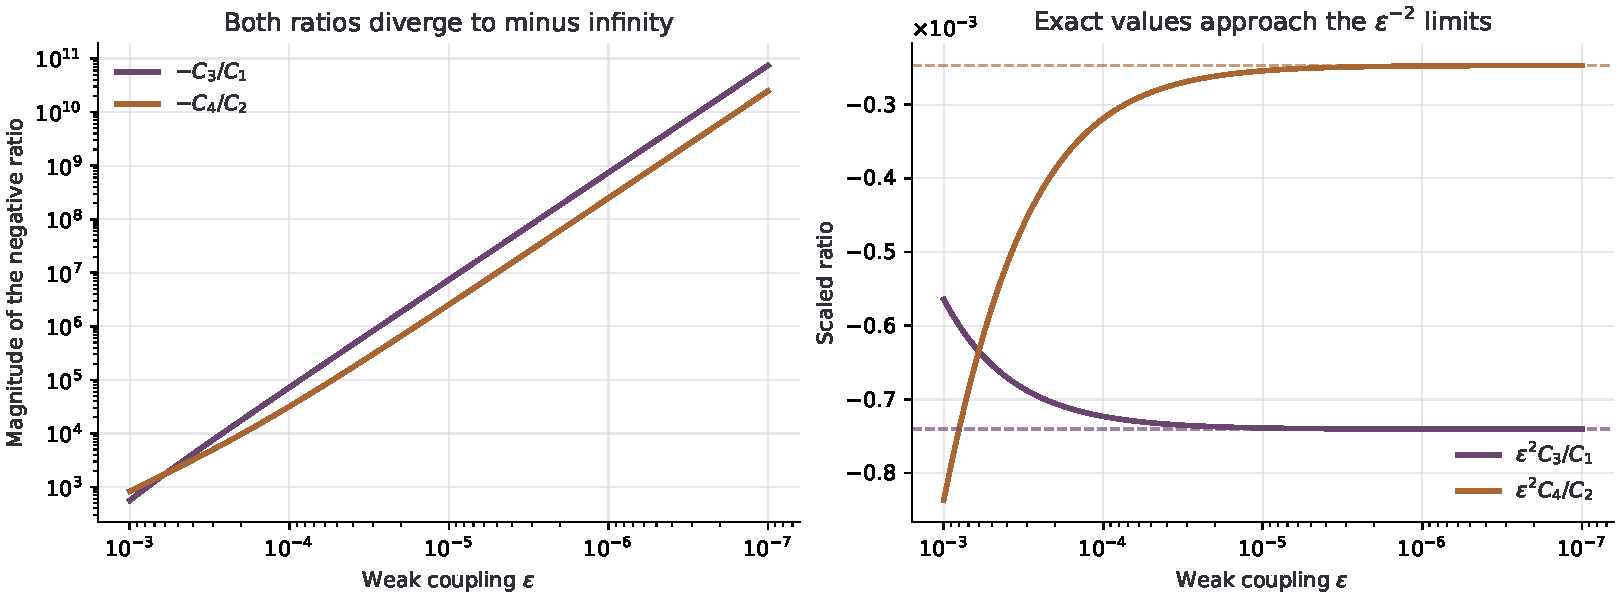
\includegraphics[width=\textwidth]{figures/thermal_divergence.pdf}
\caption{The full-support family at fixed thermodynamic data. Left: magnitudes of the two negative ratios. Right: multiplying by $\eps^2$ approaches $-16/21609$ and $-16/64827$ (dashed). $\eps$ decreases to the right. The approach of $\eps^2K$ is slow, as~\eqref{eq:laurent} predicts. Each value was computed by exact rational recursion.}
\label{fig:divergence}
\end{figure}

\section{Open problems}\label{sec:open}
\begin{enumerate}[nosep]
\item \emph{Normalised kurtosis in three states.} Is $\hat K=C_4C_1^2/C_2^3\ge-15/4$ for every three-state, two-bath thermal network? Proposition~\ref{prop:normlim} gives $-15/4$ as the infimum of the switching limit in the trap family, and Proposition~\ref{prop:product} shows that no such bound holds with six states. \emph{Numerical evidence:} across $6\times10^5$ random networks (Table~\ref{tab:census}) the smallest value was $-3.68$.
\item \emph{Sign rule under bounded disparity.} Is there an explicit $R_*$ such that $S\ge0$ and $K\ge0$ whenever the largest-to-smallest rate ratio is at most $R_*$? \emph{Numerical evidence:} no violation in the census had disparity below $99$, and the simple certificate needs disparity above $60$ for $K<0$. Compactness suggests a finite lower bound for each fixed $R$, but we have proved neither that nor an explicit sign threshold.
\item \emph{Sharp kinetic constants.} Theorem~\ref{thm:kinetic} has the right order in the gap but constants about $10^4$ too large. An activity-based or gap-based bound with sharp constants would replace the conjectures by a usable inequality.
\item \emph{Which bounds survive in the source.} The same mechanism should be tested against the source's other numerically supported inequalities, including those for unicyclic networks and more baths.
\end{enumerate}

\section*{Declarations}\sloppy
\textbf{Author.} Anonymous.\\
\textbf{AI provenance.} This manuscript, its proofs, code and figures were produced with substantial assistance from AI language models working under human direction. The revision responds to five AI-generated referee reports, a separate AI-assisted proof audit and a final AI-assisted correctness audit; none of these is human peer review. Every quantitative claim is backed by the exact or seeded computations in the supplement.\\
\textbf{Funding and competing interests.} None.\\
\textbf{Data and code.} The supplement is archived at \url{https://doi.org/10.5281/zenodo.23689958} and at \url{https://github.com/ipitchford/thermal-cumulant-sign-counterexamples} (tag \texttt{v1.0.0-candidate}), as described in Section~\ref{sec:verify}. Text CC0-1.0; code MIT.

\begingroup\small\setlength{\parskip}{2pt}
\begin{thebibliography}{99}
\bibitem{Ptaszynski2022} Ptaszy\'nski, K. (2022). Bounds on skewness and kurtosis of steady-state currents. \emph{Physical Review E, 106}, 024119. \url{https://doi.org/10.1103/PhysRevE.106.024119}.
\bibitem{BaratoSeifert2015} Barato, A. C., \& Seifert, U. (2015). Thermodynamic Uncertainty Relation for Biomolecular Processes. \emph{Physical Review Letters, 114}, 158101. \url{https://doi.org/10.1103/PhysRevLett.114.158101}.
\bibitem{Gingrich2016} Gingrich, T. R., Horowitz, J. M., Perunov, N., \& England, J. L. (2016). Dissipation Bounds All Steady-State Current Fluctuations. \emph{Physical Review Letters, 116}, 120601. \url{https://doi.org/10.1103/PhysRevLett.116.120601}.
\bibitem{BaratoSeifert2015sk} Barato, A. C., \& Seifert, U. (2015). Skewness and Kurtosis in Statistical Kinetics. \emph{Physical Review Letters, 115}, 188103. \url{https://doi.org/10.1103/physrevlett.115.188103}.
\bibitem{WamplerBarato2022} Wampler, T., \& Barato, A. C. (2022). Skewness and kurtosis in stochastic thermodynamics. \emph{Journal of Physics A: Mathematical and Theoretical, 55}, 014002. \url{https://doi.org/10.1088/1751-8121/ac3b0c}.
\bibitem{Salazar2022} Salazar, D. S. P. (2022). Thermodynamic skewness relation from detailed fluctuation theorem. \emph{Physical Review E, 106}, L042101. \url{https://doi.org/10.1103/PhysRevE.106.L042101}.
\bibitem{Esposito2009} Esposito, M., Harbola, U., \& Mukamel, S. (2009). Nonequilibrium fluctuations, fluctuation theorems, and counting statistics in quantum systems. \emph{Reviews of Modern Physics, 81}, 1665--1702. \url{https://doi.org/10.1103/RevModPhys.81.1665}.
\bibitem{Bruderer2014} Bruderer, M., Contreras-Pulido, L. D., Thaller, M., Sironi, L., Obreschkow, D., \& Plenio, M. B. (2014). Inverse counting statistics for stochastic and open quantum systems: the characteristic polynomial approach. \emph{New Journal of Physics, 16}, 033030. \url{https://doi.org/10.1088/1367-2630/16/3/033030}.
\bibitem{Jordan2004} Jordan, A. N., \& Sukhorukov, E. V. (2004). Transport statistics of bistable systems. \emph{Physical Review Letters, 93}, 260604. \url{https://doi.org/10.1103/PhysRevLett.93.260604}.
\bibitem{BagretsNazarov2003} Bagrets, D. A., \& Nazarov, Yu. V. (2003). Full counting statistics of charge transfer in Coulomb blockade systems. \emph{Physical Review B, 67}, 085316. \url{https://doi.org/10.1103/PhysRevB.67.085316}.
\bibitem{Flindt2009} Flindt, C., Fricke, C., Hohls, F., Novotn\'y, T., Neto\v{c}n\'y, K., Brandes, T., \& Haug, R. J. (2009). Universal oscillations in counting statistics. \emph{Proceedings of the National Academy of Sciences, 106}, 10116--10119. \url{https://doi.org/10.1073/pnas.0901002106}.
\bibitem{DiTerlizziBaiesi2019} Di Terlizzi, I., \& Baiesi, M. (2019). Kinetic uncertainty relation. \emph{Journal of Physics A: Mathematical and Theoretical, 52}, 02LT03. \url{https://doi.org/10.1088/1751-8121/aaee34}.
\bibitem{PtaszynskiEsposito2025} Ptaszy\'nski, K., \& Esposito, M. (2025). Critical heat current fluctuations in Curie-Weiss model in and out of equilibrium. \emph{Physical Review E, 111}, 034125. \url{https://doi.org/10.1103/PhysRevE.111.034125}.
\bibitem{Saryal2019} Saryal, S., Friedman, H. M., Segal, D., \& Agarwalla, B. K. (2019). Thermodynamic uncertainty relation in thermal transport. \emph{Physical Review E, 100}, 042101. \url{https://doi.org/10.1103/PhysRevE.100.042101}.
\bibitem{BauerFike1960} Bauer, F. L., \& Fike, C. T. (1960). Norms and exclusion theorems. \emph{Numerische Mathematik, 2}, 137--141. \url{https://doi.org/10.1007/BF01386217}.
\bibitem{Kato1995} Kato, T. (1995). \emph{Perturbation Theory for Linear Operators}. Classics in Mathematics, Springer. \url{https://doi.org/10.1007/978-3-642-66282-9}.
\end{thebibliography}
\endgroup
\end{document}
